\documentclass[a4paper,handout,mathserif,final,xcolor=dvipsnames,twocolumn]{beamer}

\useinnertheme{rectangles}
%\useoutertheme{infolines}
\usecolortheme{orchid}
\usetheme{Darmstadt}
\setbeamertemplate{blocks}[rounded][shadow=true]


\usepackage[utf8]{inputenc}
\usepackage{rotating}
\usepackage{multicol}
\usepackage{pstricks}
\usepackage{pst-node}
\usepackage{pst-plot}
\usepackage{amsmath}
\usepackage{subfigure}
%\renewcommand{\bibsection}{\subsubsection*{\bibname } }
\usepackage{natbib}

\newtheorem{thm}{Theorem}[section]
\newtheorem{cor}[thm]{Corollary}
\newtheorem{proposition}[thm]{Proposition}
\newtheorem{condition}[thm]{Buchanan}



\title{Economía política, federalismo y elecciones en Argentina}
\author{Sebastián Freille}
 \institute{\inst{1}FCE/UNC y CICE/UNC-CONICET \\ XVIII Encuentro de
 Geografías de América Latina}}
\date{Noviembre 2021}

\usepackage{epigraph}

\begin{document}
\maketitle

%\section{Dinero, elecciones y políticas}



% \section{Motivación}


%   \begin{frame}\frametitle{Contexto}
% \begin{itemize}\itemsep 15pt 
% \item Existen diferentes dimensiones del federalismo:
%   \begin{itemize} \medskip
%   \item Económica $\longrightarrow$ asignativo, financiero
%   \item Política $\longrightarrow$ electoral, coalicional
%   \item Administrativa $\longrightarrow$ burocracia, implementación
%     \end{itemize}

% \item Tradicionalmente estos aspectos han sido estudiados por separado
%   --i.e. economía estudiaba aspectos de asignación/provisión óptima de
%   funciones entre
%   niveles; externalidades [Oates (1972, 1999), Tiebout
%   (1965), Inman and Rubinfeld (1992); la ciencia política
%   estudiaba las instituciones políticas en los diferentes niveles
%   [Riker (1964), Weingast (1995), Iaryczower, Saiegh and Tommassi
%   (1999), Persson and Tabellini (1996), Gibson and Calvo (2000)
% \end{itemize}
% \end{frame}





% \begin{frame}\frametitle{Contexto (cont.)}
% \begin{itemize}
% \item En los sistemas multi-nivel, se eligen representantes en
%     diferentes niveles de gobierno --nacional, provincial, local;
%     co-existen diferentes sistemas, reglas y arreglos electorales.
%     \item ¿Pueden estas diferencias tener efectos sobre la forma en que
%       políticos de diferente nivel interactúan? ¿Condicionan estas
%       diferencias el accionar de los diferentes representantes en un
%       país federal? ¿Tiene esto asociados impactos coyunturales y
%       estructurales?
%       \item La propuesta en este punto es dejar planteados estos temas
%         y examinar alguna evidencia anecdótica y empírica que nos
%         permita abordar el tema en forma mas analítica.
%       \end{itemize}
%       \end{frame}

%       \begin{frame}\frametitle{Algunos ejes de la discusión}
%         \begin{itemize}
%         \item Aspectos del federalismo político
%           \begin{itemize}\itemsep 5pt \medskip
%           \item Fragmentación partidaria en diferentes niveles
%             \item Desnacionalización de partidos
%           \item Alineación de resultados electorales de
%             ``oficialismos'' de diferente nivel
%           \end{itemize}
%           \item Un tema relevante es como se relaciona las elecciones para
%   diferentes niveles. En otros términos, cómo electores de un mismo
%   distrito eligen diferentes cargos y qué impacto tiene esto. 
% \item Tema relacionado $\longrightarrow$ externalidades
%   ``electorales'' (spillover effects aka ``coattails''). 
% \end{itemize}
%           \end{frame}

          
\section{Fragmentación partidaria}


\begin{frame}\frametitle{El diseño institucional del federalismo político}
  \begin{itemize}\itemsep 10pt
    \item Los sistemas y reglas de elección de representates suelen
      variar en una federación.
      \begin{itemize}\itemsep 5pt \smallskip
        \item El ejecutivo nacional(Presidente) en Argentina se elige a través de un  \textbf{sistema mayoritario de doble vuelta (``ballotage'')}
          \item Los ejecutivos provinciales (gobernadores) se eligen
            usando sistemas diferentes:
            \begin{itemize}\itemsep 5pt \smallskip
            \item Los gobernadores de Chaco, Corrientes
              y Tierra del Fuego se eligen con un \textbf{sistema mayoritario
              de doble vuelta (``ballotage'')}
              \item Formosa y Jujuy combinan el \textbf{sistema de simple
                pluralidad con ley de Lemas}.
                \item El resto de las provincias tienen un \textbf{sistema de
                  simple pluralidad}. 
            \end{itemize}
            \item El legislativo nacional se
              eligen a través un de \textbf{sistema de representación
              proporcional} y un \textbf{sistema mayoritario con lista
              incompleta}.
            \end{itemize}
\end{itemize}
          \end{frame}


\begin{frame}\frametitle{Las ``leyes'' de Duverger}
 \begin{block}{Ley 1}
Los sistemas de votación por mayoría en una elección conducen a un sistema bipartidista
\end{block}
\begin{block}{Ley 2}
Los sistemas de votación por representación proporcional conducen a un
sistema multipartidista. 
\end{block}
\begin{block}{Ley 3}
Los sistemas de votación por mayoría en dos vueltas (``ballotage'') conducen a un
sistema multipardista con tendencia a formar coaliciones
\end{block}
  \end{frame}

  
  \begin{frame}\frametitle{La situación en Argentina}
    \begin{itemize}\itemsep 10pt
    \item Si estas ``leyes'' tienen algun sustento empírico, uno
      debería observar en un país como Argentina lo siguiente:
      \begin{itemize}\itemsep 5pt \smallskip
      \item En elecciones ejecutivas nacionales, un sistema
        multipartido con tendencia a formar coaliciones de gobierno
                \item En elecciones legislativas nacionales, un
                  sistema multipartido
                  \item En elecciones ejecutivas sub-nacionales, un
                    sistema compuesto por un mix entre sistemas
                    bipartidistas y multi-partidistas con coaliciones
                  \end{itemize}
\item Una medida muy usada para capturar el diferente grado de
  fragmentación de partidos es el \textbf{numero efectivo de partidos}
  \begin{equation*}
NEP=\frac{1}{\sum_{i=1}^{n}v_{i}^2}
    \end{equation*}
      \end{itemize}
  \end{frame}


  \begin{frame}\frametitle{La situación en Argentina (cont.)}
 \begin{figure}[htbp]
    \centering 
    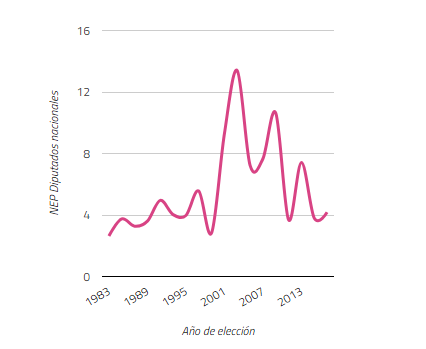
\includegraphics[scale=0.675]{grafico2}
    \caption{Número efectivo de partidos, Diputados (Fuente: CIPPEC)}
    \label{fig:1}
  \end{figure}
    \end{frame}


 \begin{frame}\frametitle{La situación en Argentina (cont.)}
 \begin{figure}[htbp]
    \centering
    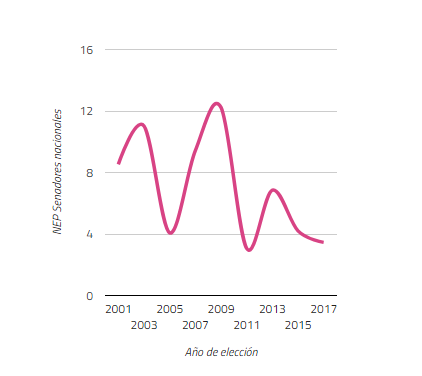
\includegraphics[scale=0.625]{grafico3}
    \caption{Número efectivo de partidos, Senadores (Fuente: CIPPEC)}
    \label{fig:1}
  \end{figure}
    \end{frame}


 \begin{frame}\frametitle{La situación en Argentina (cont.)}
 \begin{figure}[htbp]
    \centering \vspace{-0.25cm}
    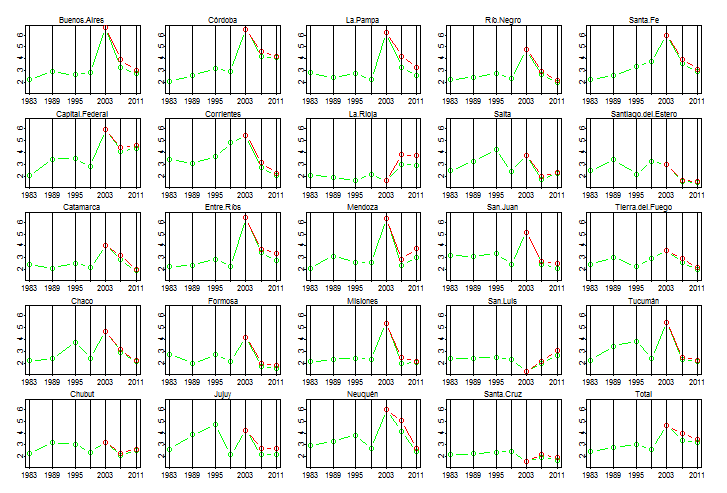
\includegraphics[scale=0.35]{grafico4}
    \caption{Número efectivo de partidos, Gobernadores (Fuente:
      Escolar y Calvo (2005), actualizado}
    \label{fig:1}
  \end{figure}
    \end{frame}


    \begin{frame}\frametitle{Fragmentación partidaria y coaliciones estables}
      \begin{itemize}\itemsep 10pt
        \item Un alto grado de fragmentación partidaria entra en
          cierto conflicto con un sistema presidencialista
          (inexistencia de mecanismos institucionales para la
          formación de coaliciones)
          \item En esta situación, y acoplado con los diferente
            sistemas electorales mencionados, habrá probabilidades de
            tener situaicones de \textbf{ejecutivo nacional con bajo
              apoyo electoral} con un
            \textbf{legislativo nacional fragmentado y opositor} y \textbf{gobernadores
              con alto apoyo electoral.}
            \item En estas condiciones, surge un contexto en el que
              los ejecutivos nacionales y gobernadores provinciales
              entran en un juego potencial de ganar-ganar por medio de
              acuerdos económico-políticos. 
            \end{itemize}
      \end{frame}

      
\section{Alineación de resultados electorales}
          
\begin{frame}\frametitle{Elecciones y porcentajes}
  \begin{figure}[htbp]
    \centering \vspace{-0.5cm}
    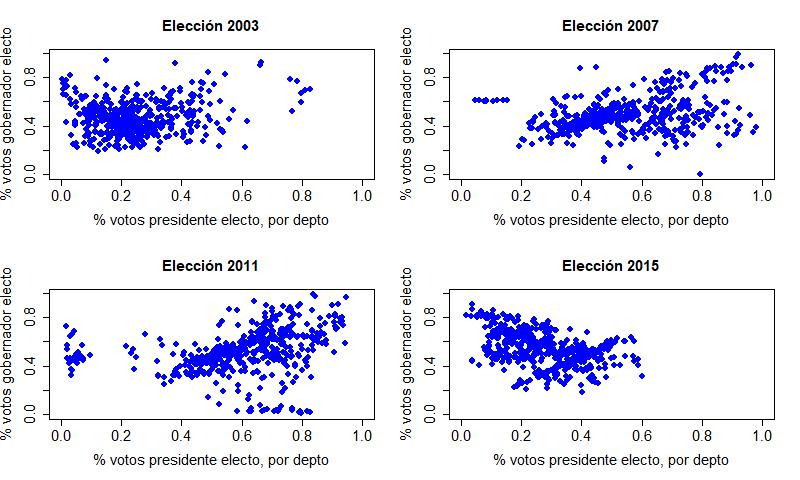
\includegraphics[scale=0.375]{correlacion2}
    \caption{Correlación de \% de votos, Presidente y Gobernador}
    \label{fig:1}
  \end{figure}
\end{frame}


\begin{frame}\frametitle{Elecciones y porcentajes (cont.)}
  \begin{figure}[htbp]
    \centering \vspace{-0.25cm}
    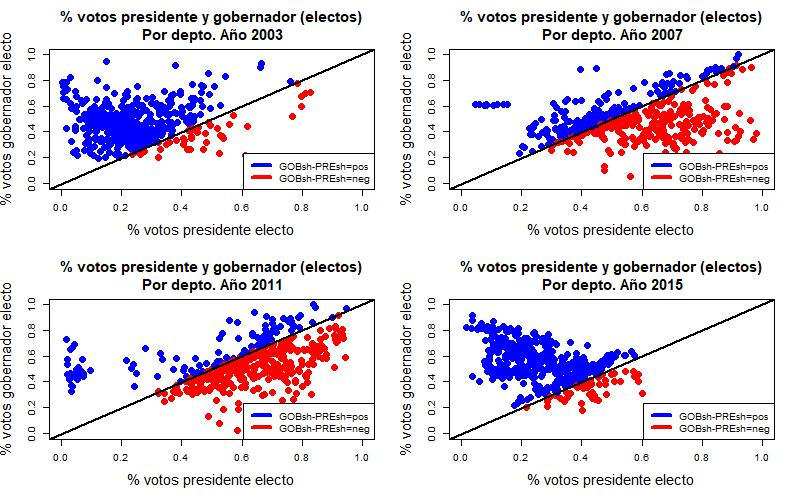
\includegraphics[scale=0.375]{coattails1}
    \caption{Correlación de \% de votos, Presidente y Gobernador, por
      Depto ``ganado''}
    \label{fig:1}
  \end{figure}
\end{frame}


% \begin{frame}\frametitle{Elecciones y porcentajes (cont.)}
%   \begin{figure}[htbp]
%     \centering \vspace{-0.25cm}
%     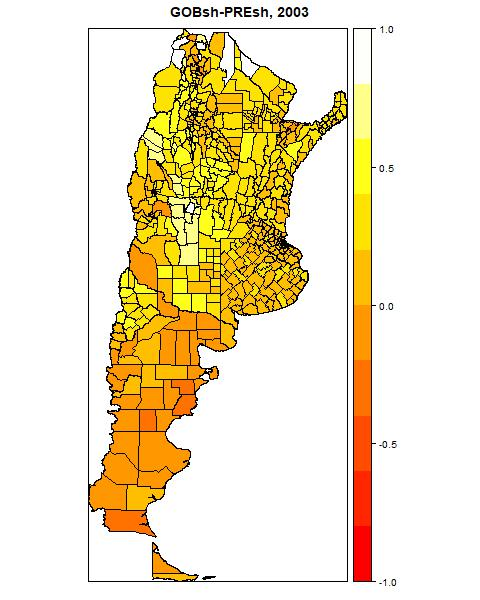
\includegraphics[scale=0.35]{map2003}
%     \caption{Mapa de intensidades de votos (en diferencia), Presidente
%       y Gobernador, 2003}
%     \label{fig:1}
%   \end{figure}
% \end{frame}


% \begin{frame}\frametitle{Elecciones y porcentajes (cont.)}
%   \begin{figure}[htbp]
%     \centering \vspace{-0.25cm}
%     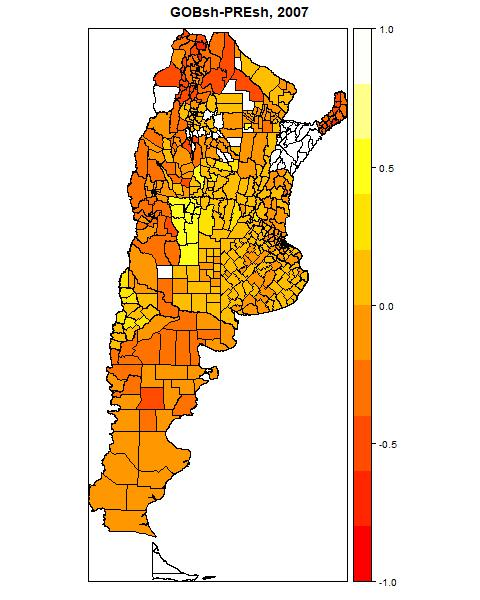
\includegraphics[scale=0.35]{map2007}
%     \caption{Mapa de intensidades de votos (en diferencia), Presidente
%       y Gobernador, 2007}
%     \label{fig:1}
%   \end{figure}
% \end{frame}


% \begin{frame}\frametitle{Elecciones y porcentajes (cont.)}
%   \begin{figure}[htbp]
%     \centering \vspace{-0.25cm}
%     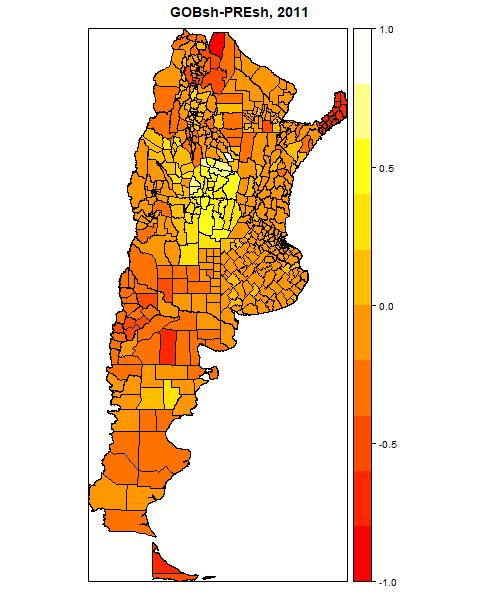
\includegraphics[scale=0.35]{map2011}
%     \caption{Mapa de intensidades de votos (en diferencia), Presidente
%       y Gobernador, 2011}
%     \label{fig:1}
%   \end{figure}
% \end{frame}


% \begin{frame}\frametitle{Elecciones y porcentajes (cont.)}
%   \begin{figure}[htbp]
%     \centering \vspace{-0.25cm}
%     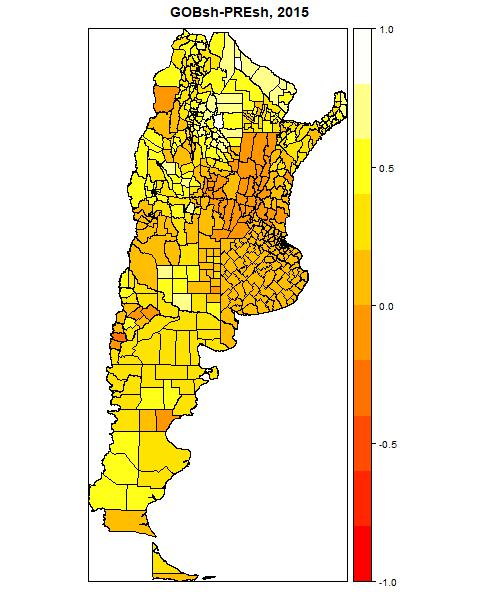
\includegraphics[scale=0.35]{map2015}
%     \caption{Mapa de intensidades de votos (en diferencia), Presidente
%       y Gobernador, 2015}
%     \label{fig:1}
%   \end{figure}
% \end{frame}


\begin{frame}\frametitle{Elecciones y porcentajes (cont.)}
  \begin{figure}
  \centering
  \subfigure[]{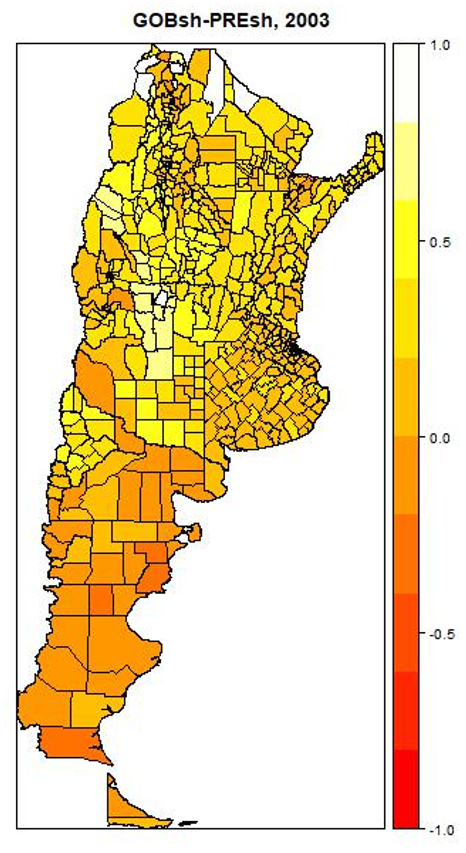
\includegraphics[width=0.24\textwidth]{map2003_v2}}
  \subfigure[]{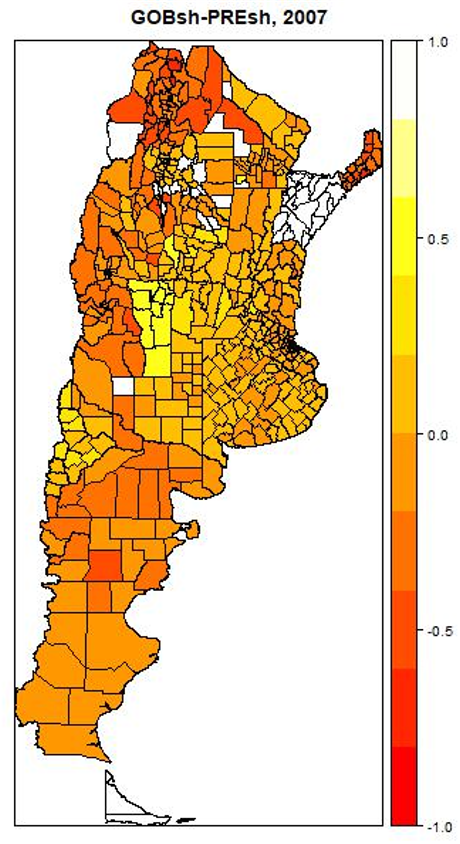
\includegraphics[width=0.24\textwidth]{map2007_v2}}
  \subfigure[]{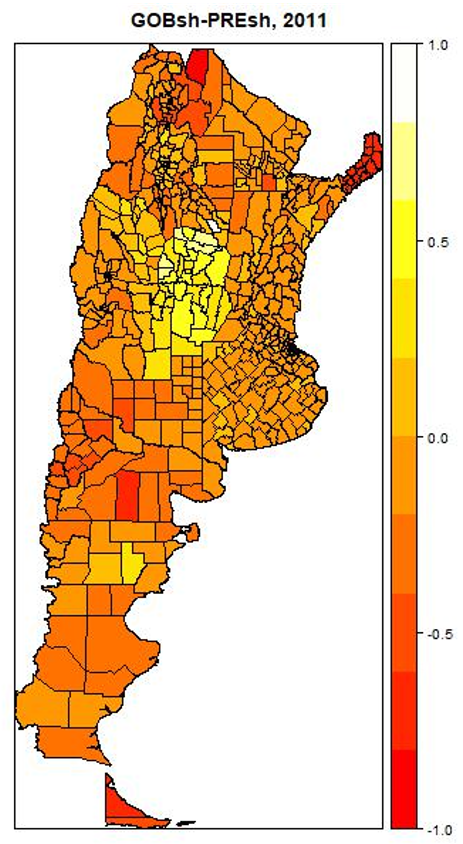
\includegraphics[width=0.24\textwidth]{map2011_v2}}
  \subfigure[]{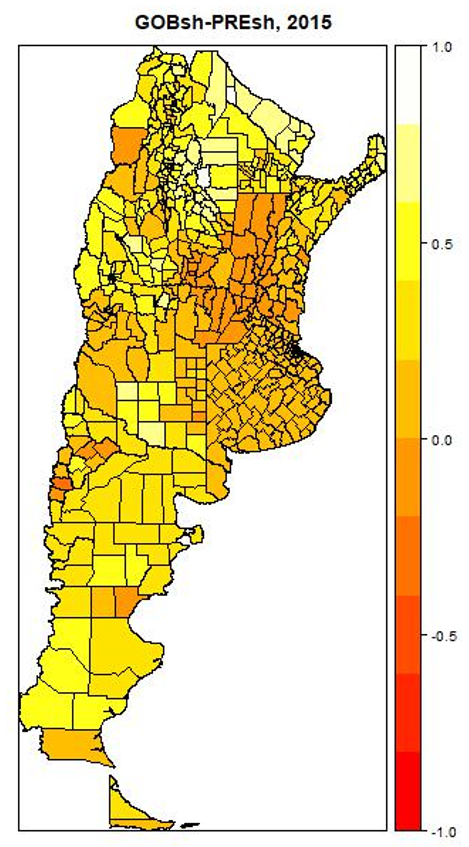
\includegraphics[width=0.24\textwidth]{map2015_v2}}
  \caption{Difference between vote shares of winning governor and President}
    \label{fig:foobar}
    \end{figure}
  \end{frame}



\begin{frame}\frametitle{``Liga de Gobernadores''}
  \begin{itemize}\itemsep 10pt
  \item Esta figura que reaparece en las discusiones sobre las
    relaciones entre Nación y provincias tiene algunas características
    particulares.
    \begin{itemize}
    \item No distingue según colores políticos
      \item Intercambia fondos de Nación por lealtades políticas de
        gobiernos sub-nacionales en dos niveles: nivel parlamentario,
        con apoyoy legislativo; nivel electoral, con maquinaria
        electoral territorial
        \item ``No los une el amor sino el espanto''
     \end{itemize}
    \item Alta dependencia financiera de muchas provincias; otras
      provincias tienen situaciones con transferencia de cajas previsionales
    \end{itemize}
  \end{frame}

  \begin{frame}\frametitle{Dependencia del gobierno nacional}
\begin{figure}[htbp]
    \centering \vspace{-0.5cm}
    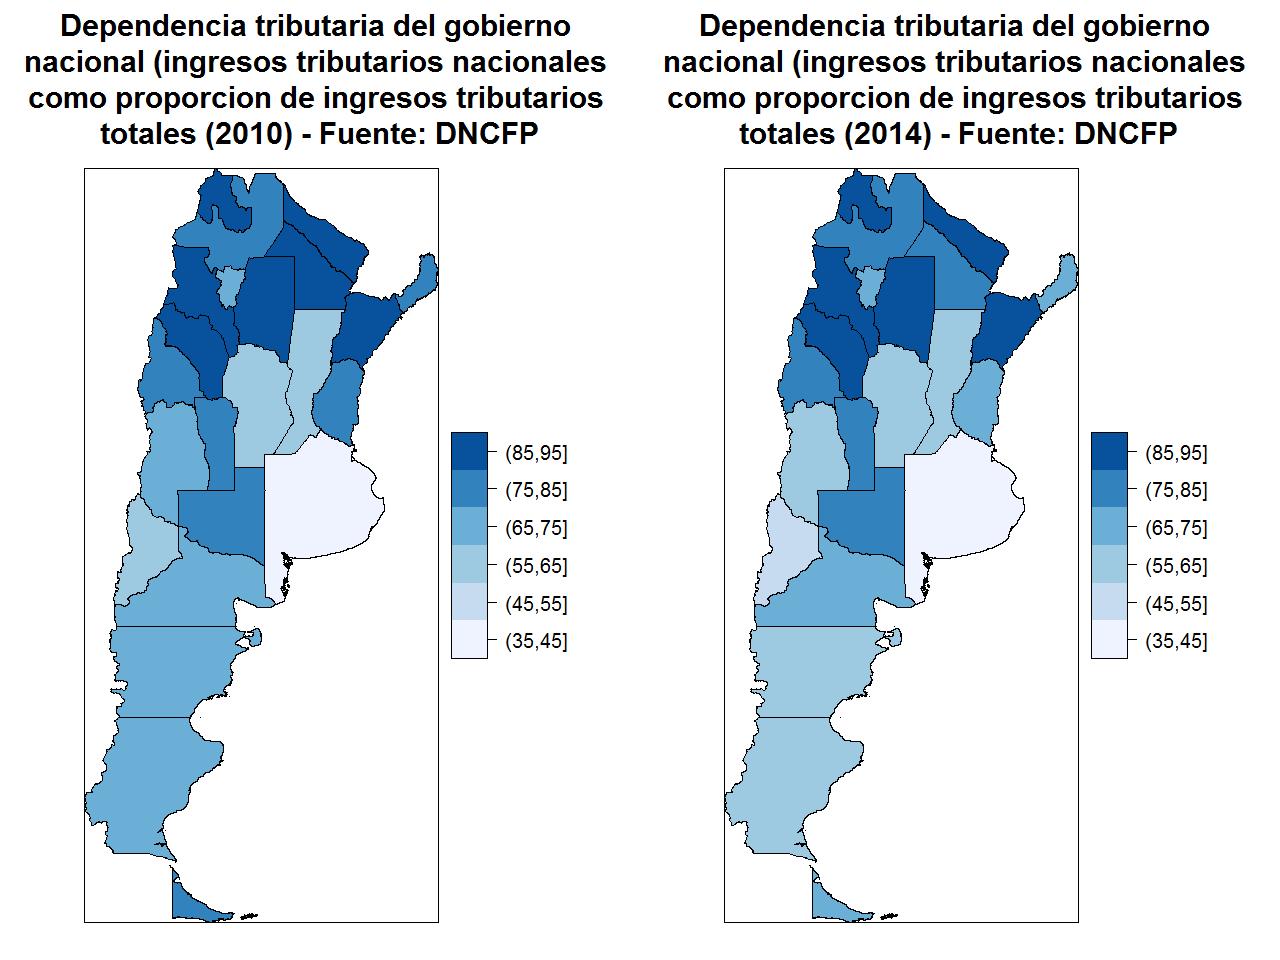
\includegraphics[scale=0.375]{grafico5}
    \caption{Dependencia tributaria de la Nación}
    \label{fig:1}
  \end{figure}
    \end{frame}
  
    \section{``Coattails'' y elecciones concurrentes}

    \begin{frame}\frametitle{``Coattails'' y elecciones concurrentes}
  \begin{itemize}\itemsep 10pt
  \item Algunos autores sugieren que existe una correlación entre los
    votos obtenidos para diferentes cargos electivos y que resulta de
    ``ir pegado'' a la misma boleta en el mismo dia de elección
    $\longrightarrow$ presidente y legisladores nacionales (ejemplo
    clásico); presidente y gobernador (en países federales)
    \item Resulta interesante examinar empíricamente si hay algún tipo
      de efecto y en qué direccion se da
      \item Usamos los mismos datos anteriores pero aclarando que
        ahora tomaremos una variable ``core'' que tiene que ver con la
        pertenencia (del gobernador electo) a la coalición nacional gobernante 
    \end{itemize}
  \end{frame}
    


\begin{frame}\frametitle{Analisis}
  \begin{itemize}\itemsep 10pt
                  \item Esto podría resultar en múltiples escenarios
                    en cuanto a la distribución de poder
                    político/electoral entre los diferentes cargos que
                    resulta interesante estudiar.
                    \item Implicancias para diseño institucional
                      $\longrightarrow$ incentivos para modificar
                      instituciones políticas a nivel nacional y
                      provincial
                      \item ¿Nueva Ley de Coparticipación?
                        $\longrightarrow$ dificil desarticular
                        incentivos para continuar con este esquema
                        ``ganar-ganar'' que se articula entre
                        presidentes y gobernadores. 
                  \end{itemize}
                \end{frame}



 \begin{frame}

% Table created by stargazer v.5.1 by Marek Hlavac, Harvard University. E-mail: hlavac at fas.harvard.edu
% Date and time: vie, ago 14, 2015 - 03:08:39 a.m.
% Requires LaTeX packages: dcolumn
\begin{table}[!htbp] \centering
\renewcommand{\arraystretch}{0.8}
\scriptsize
\begin{tabular}{@{\extracolsep{5pt}}lcccc}
\\[-1.8ex]\hline
 & \multicolumn{4}{c}{\textit{Dependent variable: Presidential Vote
   Share [Pooled OLS]}} \\
\cline{2-5} \\
 shgob & -0.87^{***} & -0.80^{***} & -0.07^{**} & -0.46^{***} \\
  & (0.05) & (0.05) & (0.03) & (0.05) \\
 core & -0.26^{***} & -0.21^{***} &  & -0.02 \\
  & (0.03) & (0.03) &  & (0.03) \\
 ENCPrez & -0.11^{***} & -0.11^{***} & -0.10^{***} & -0.09^{***} \\
  & (0.002) & (0.002) & (0.004) & (0.003) \\
 conc &  & -0.07 & -0.11^{**} & 0.54^{***} \\
  &  & (0.04) & (0.06) & (0.07) \\
\textcolor{blue}{days} &  & -0.0004 & -0.03^{***} & -0.03^{***} \\
  &  & (0.01) & (0.01) & (0.01) \\
  shgob:core & 1.00^{***} & 0.86^{***} &  & 0.45^{***} \\
  & (0.05) & (0.05) &  & (0.06) \\
 shgob:conc &  & 0.12^{**} &  & -1.26^{***} \\
  &  & (0.05) &  & (0.12) \\
 core:conc &  &  &  & -0.83^{***} \\
  &  &  &  & (0.07) \\
\textcolor{blue}{shgob:core:conc} &  &  &  & 1.56^{***} \\
  &  &  &  & (0.13) \\
 pubemp &  &  & 0.003^{***} & 0.003^{***} \\
  &  &  & (0.0003) & (0.0002) \\
  conc:shgob &  &  & 0.05 &  \\
  &  &  & (0.06) &  \\
\hline
Observations & \multicolumn{1}{c}{1,390} & \multicolumn{1}{c}{1,301} & \multicolumn{1}{c}{1,240} & \multicolumn{1}{c}{1,240} \\
Adjusted R$^{2}$ & \multicolumn{1}{c}{0.74} & \multicolumn{1}{c}{0.76} & \multicolumn{1}{c}{0.66} & \multicolumn{1}{c}{0.81} \\
F Statistic & \multicolumn{1}{c}{1,010.10$^{***}$} & \multicolumn{1}{c}{596.12$^{***}$} & \multicolumn{1}{c}{395.51$^{***}$} & \multicolumn{1}{c}{545.26$^{***}$} \\
\hline
\textit{Note:}  & \multicolumn{4}{r}{$^{*}$p$<$0.1; $^{**}$p$<$0.05; $^{***}$p$<$0.01} \\
\end{tabular}
\end{table}
\end{frame}



\begin{frame}

% Table created by stargazer v.5.1 by Marek Hlavac, Harvard University. E-mail: hlavac at fas.harvard.edu
% Date and time: vie, ago 14, 2015 - 02:18:37 a.m.
\begin{table}[!htbp] \centering
\renewcommand{\arraystretch}{0.8}
\scriptsize
\begin{tabular}{@{\extracolsep{5pt}}lcccc}
\\[-1.8ex]\hline
\hline \\[-1.8ex]
 & \multicolumn{4}{c}{\textit{Dependent variable: Presidential Vote
   Share [Panel FE, time effects]}} \\
\cline{2-5}
\hline \\[-1.8ex]
 shgob & -0.77^{***} & -0.79^{***} & -1.17^{***} & -0.44^{***} \\
  & (0.07) & (0.05) & (0.09) & (0.05) \\
 core & -0.23^{***} & -0.25^{***} & -0.41^{***} & -0.02 \\
  & (0.03) & (0.03) & (0.05) & (0.03) \\
 conc &  &  &  & 0.54^{***} \\
  &  &  &  & (0.07) \\
 ENCPrez & -0.10^{***} & -0.09^{***} & -0.17^{***} & -0.09^{***} \\
  & (0.003) & (0.003) & (0.01) & (0.003) \\
 PREZ\_FPV\_pre &  &  & 0.26^{***} &  \\
  &  &  & (0.04) &  \\
 \textcolor{blue}{days} &  &  &  & -0.03^{***} \\
  &  &  &  & (0.01) \\
 pubemp &  &  &  & 0.003^{***} \\
  &  &  &  & (0.0002) \\
 shgob:core & 1.00^{***} & 0.94^{***} & 1.19^{***} & 0.44^{***} \\
  & (0.07) & (0.05) & (0.09) & (0.06) \\
 shgob:conc &  &  &  & -1.20^{***} \\
  &  &  &  & (0.12) \\
 core:conc &  &  &  & -0.82^{***} \\
  &  &  &  & (0.07) \\
\textcolor{blue}{shgob:core:conc} &  &  &  & 1.53^{***} \\
  &  &  &  & (0.13) \\
 \hline \\[-1.8ex]
Observations & \multicolumn{1}{c}{1,390} & \multicolumn{1}{c}{1,390} & \multicolumn{1}{c}{357} & \multicolumn{1}{c}{1,240} \\
Adjusted R$^{2}$ & \multicolumn{1}{c}{0.49} & \multicolumn{1}{c}{0.54} & \multicolumn{1}{c}{0.80} & \multicolumn{1}{c}{0.64} \\
F Statistic & \multicolumn{1}{c}{684.62$^{***}$} & \multicolumn{1}{c}{416.90$^{***}$} & \multicolumn{1}{c}{309.84$^{***}$} & \multicolumn{1}{c}{228.07$^{***}$} \\
\hline
\hline \\[-1.8ex]
\textit{Note:}  & \multicolumn{4}{r}{$^{*}$p$<$0.1; $^{**}$p$<$0.05; $^{***}$p$<$0.01} \\
\end{tabular}
\end{table}
\end{frame}


\begin{frame}\frametitle{``Coattails'' (cont.)}
  \begin{itemize}\itemsep 10pt
  \item El porcentaje de votos obtenido por el presidente está
    fuertemente asociado con el porcentaje de votos obtenido por el
    gobernador en un mismo distrito (distinta elección) \textbf{solo
      si} pertenecen a la coalición del presidente.
    \item Pero el resultado mas fuerte es para aquellas elecciones que
      ocurren en la misma fecha $\longrightarrow$ es decir, estaría
      indicando evidencia de un fuerte efecto ``coattail'' (efecto
      arrastre) [aunque no puede conocerse el sentido de la
      dirección/causalidad]
      \item Finalmente, existe evidencia de que el porcentaje de votos
        del presidente está inversamente relacionado con la distancia
        entre la fecha de su elección y la del gobernador. 
    \end{itemize}
  \end{frame}


\end{document}
  
\section{Implicancias}

\begin{frame}\frametitle{Implicancias}
  \begin{itemize}\itemsep 10pt
  \item Los aspectos políticos del federalismo argentino parecen ser
 (a priori) teóricamente   relevantes en la consideración de aspectos
 económicos del federalismo argentino $\longrightarrow$ dificultad
 para acordar una nueva ley de coparticipación; permanencia de
 soluciones parciales y ``parches''
 \item Cuestión importante $\longrightarrow$ ¿cómo construyen poder
local los presidentes? Múltiples canales: a) transferencias y
subsidios directos; b) transferencias y subsidios indirectos; c) gasto
públic nacional directo (provisión de bienes y servicios;
infraestructura)
\item ¿Que aspectos del diseño institucional actual (instituciones
  políticas) pueden pensar en cambiarse para compatibilizar los
  incentivos económicos y políticos en el actual esquema del
  federalismo argentino?
    \end{itemize}
  \end{frame}
                
                
\end{document}

  

  
\begin{frame}\frametitle{Correlations}
  \begin{figure}[htbp]
    \centering
    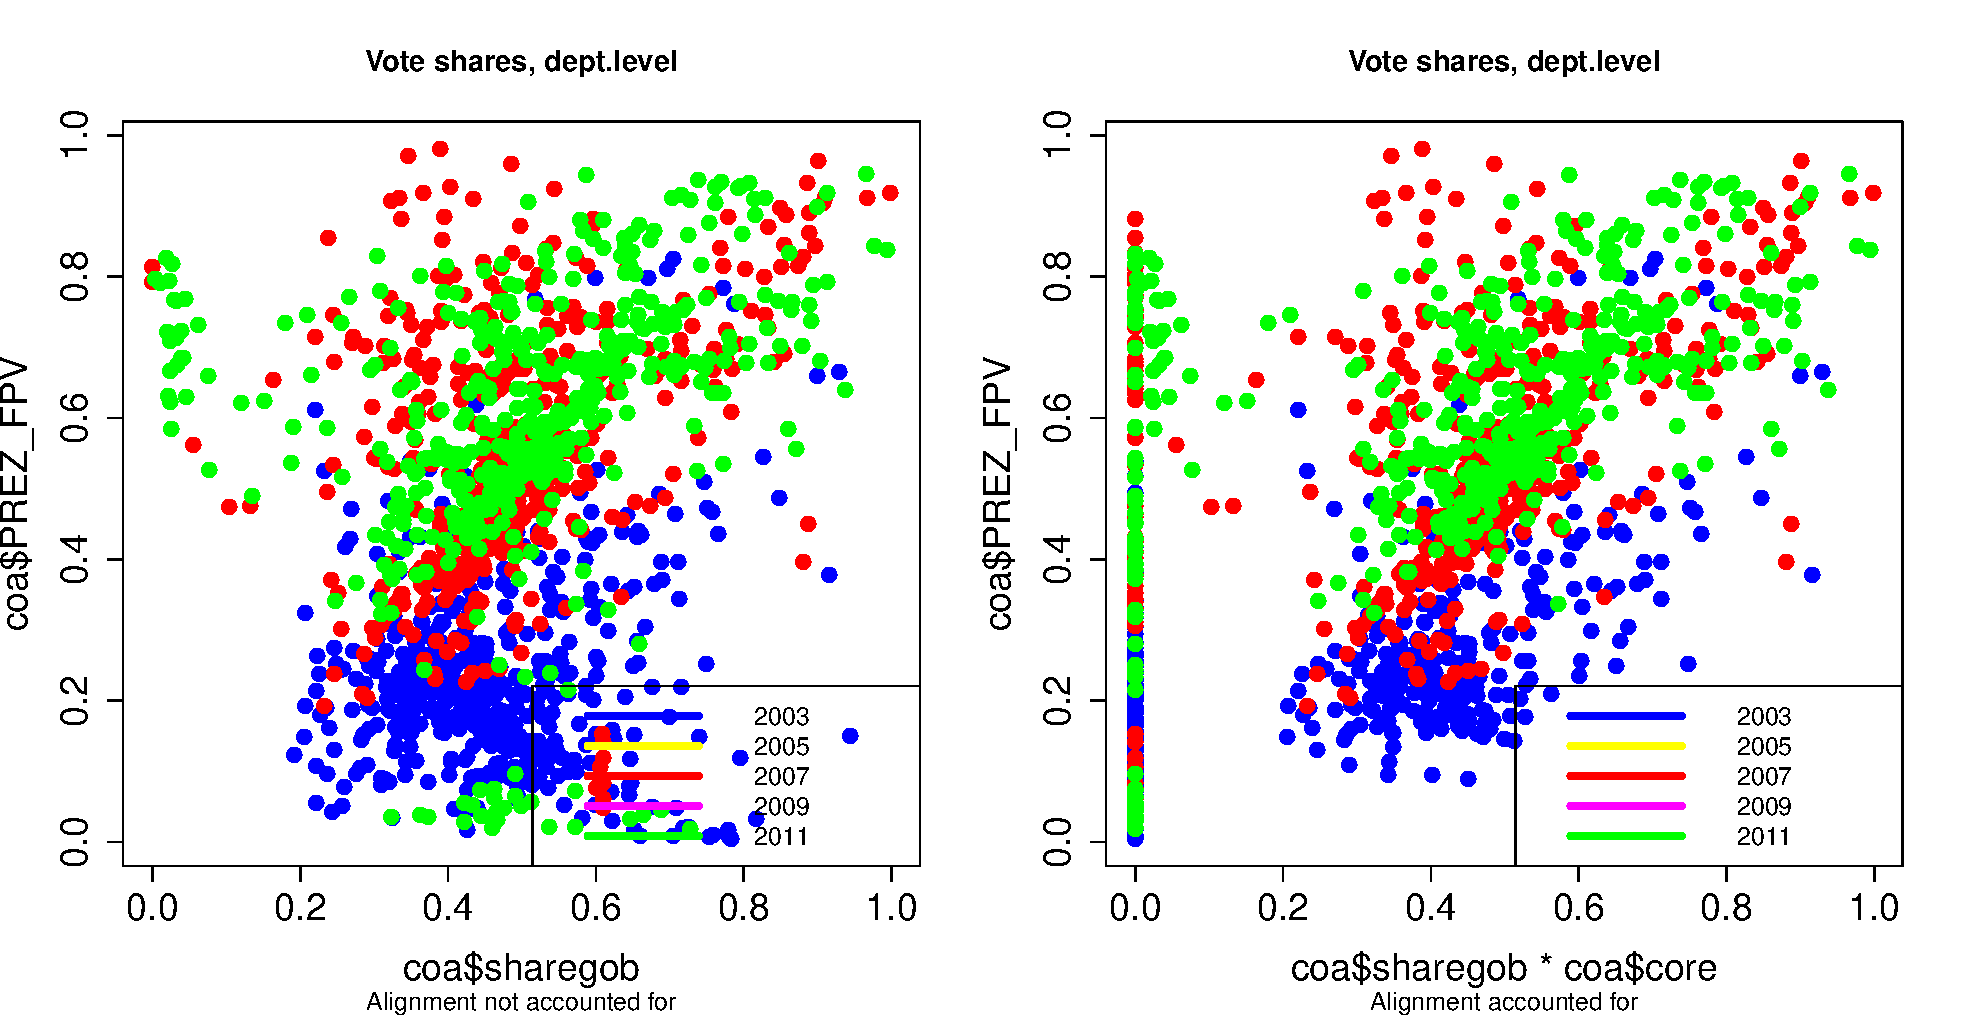
\includegraphics[scale=0.34]{int1}
    \caption{Correlation of vote shares (vertical)}
    \label{fig:1}
  \end{figure}
\end{frame}


\begin{frame}\frametitle{Correlaciones votos (cont.)}
  \begin{figure}[htbp]
    \centering
    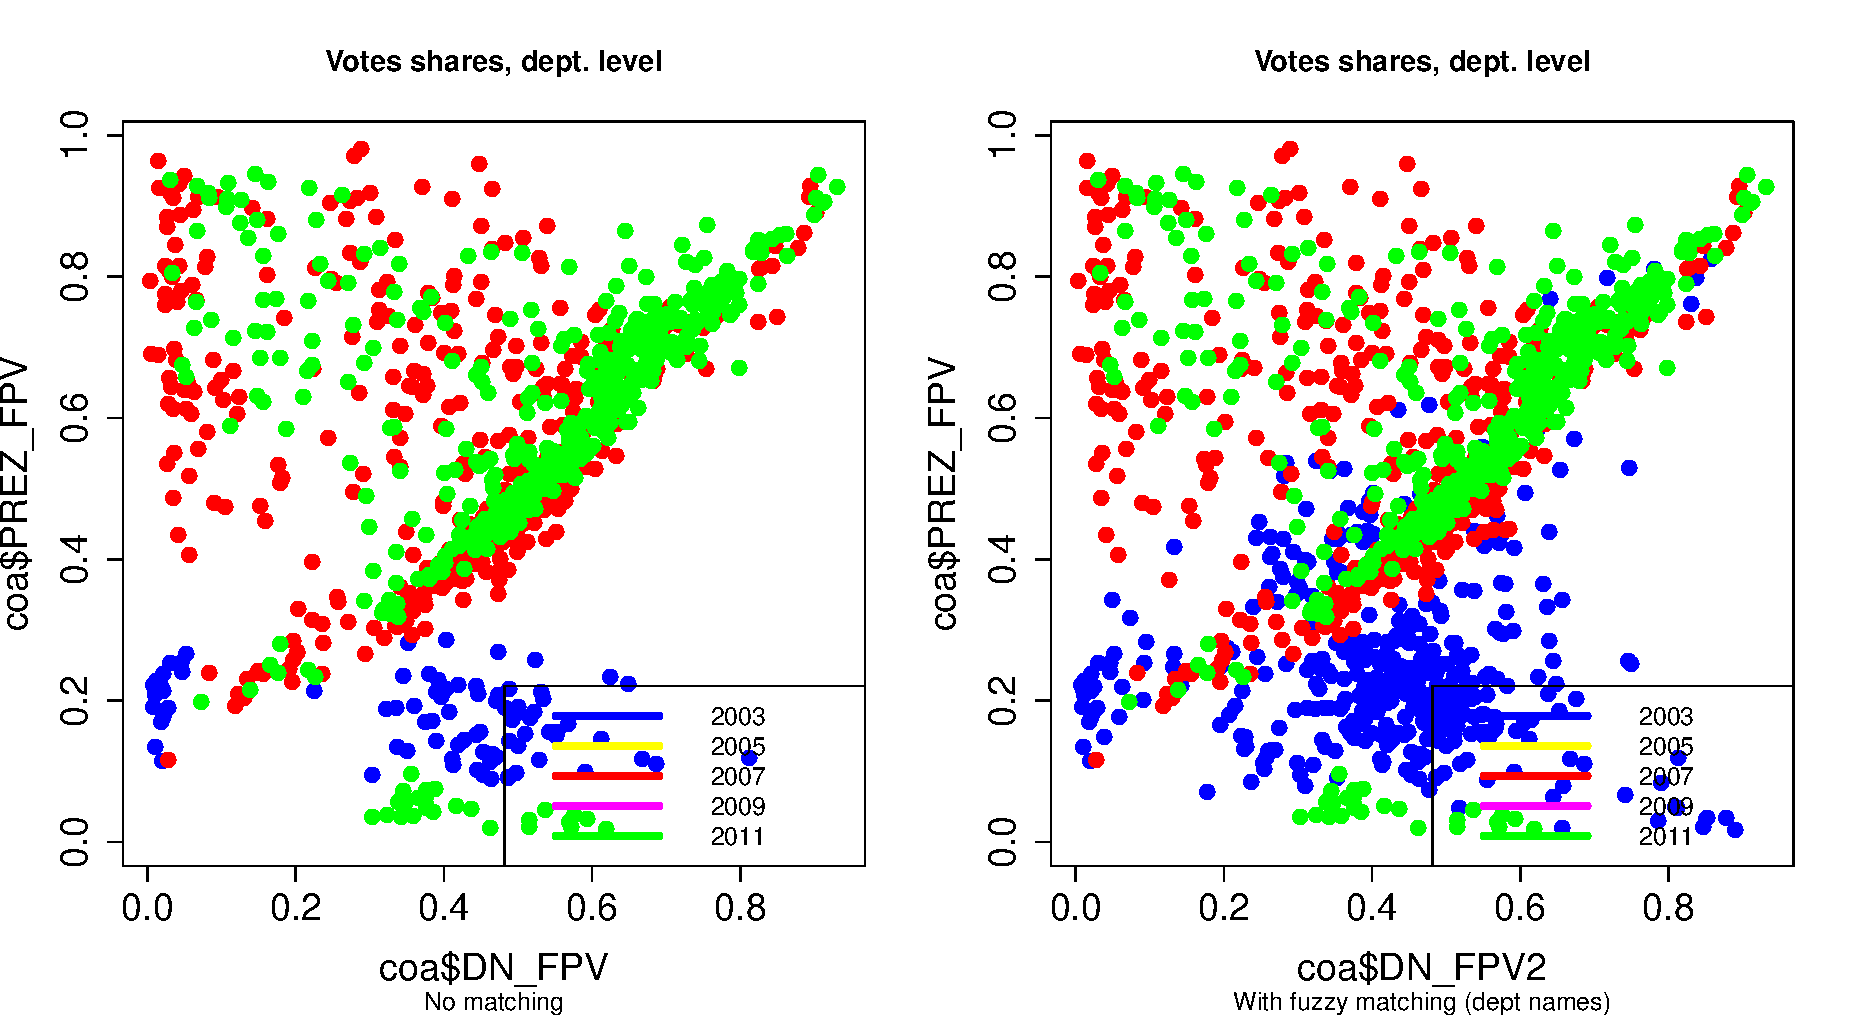
\includegraphics[scale=0.34]{int2}
    \caption{Correlation of vote shares (vertical)}
    \label{fig:1}
  \end{figure}
\end{frame}





\begin{frame}\frametitle{Where the literature stands}
\begin{itemize}\itemsep 15pt
\item  Early work studied these electoral effects [\cite{calvert1983},
\cite{ferejohn1984}, \cite{ames1994}, \cite{shugart1995}]
\item More recent work has looked at more rigorous modelling of
  coattail effects  \cite{samuels2000},
\cite{hogan2005}, \cite{oliveros}, \cite{magar2012}, \cite{meredith2013}]
\end{itemize}
\end{frame}

\section{Theory and modelling}
\begin{frame}\frametitle{Some theoretical considerations}
\begin{itemize}\itemsep 15pt
\item Why do these effects arise?:
\begin{itemize} \itemsep 15pt
\item Due to institutional design $\longrightarrow$ ballot designs
  that include a straight-ticket voting may induce larger spillovers
  (coattails)
\item Due to mobilization of party supporters $\longrightarrow$
  particularly relevant in separate elections \cite{meredith2013}
\item Due nationalization/congruence of party system $\longrightarrow$
  homogeneous votes across parties for different elections
\end{itemize}
\end{itemize}
\end{frame}


\begin{frame}\frametitle{Modeling}
\begin{itemize}\itemsep 15pt
\item We follow \cite{shugart1995} in modeling a delayed effect
$\longrightarrow$ only a empirical question [Theory is unclear, both
arguments are likely]
\item Controlling for this is possible and desirable in Argentina
  $\longrightarrow$ normally the delay between elections is less than
  6 months [average distance over three elections equals 80 days]
\item Including a variable measuring for distance between different
  elections makes sense to capture this effect.
\end{itemize}
\end{frame}


\begin{frame}\frametitle{Modeling (cont.)}
\begin{itemize}\itemsep 15pt
\item Assume that there are $n$ sub-national autonomous districts and $one$
  national government. The national government sets the election date
  exogenously. Each subnational government decides upon the date of
  election which can be: 1) before; 2) on the same date; 3) after the
  national date.
\item The decision depends on two factors: 1) the observed intra-party
  ``vertical'' vote deficit in the previous election; 2) the observed
  inter-party district-level margin of victory.
\item The timing of the game is as follows: 1) NatGov chooses elec
  date; 2) each LocGov sets its own elec date; 3) all elections take
  place; 4) each government gets payoff.
\end{itemize}
\end{frame}


\section{Data and results}

\begin{frame}

% Table created by stargazer v.5.1 by Marek Hlavac, Harvard University. E-mail: hlavac at fas.harvard.edu
% Date and time: vie, ago 14, 2015 - 03:08:39 a.m.
% Requires LaTeX packages: dcolumn
\begin{table}[!htbp] \centering
\renewcommand{\arraystretch}{0.8}
\scriptsize
\begin{tabular}{@{\extracolsep{5pt}}lcccc}
\\[-1.8ex]\hline
 & \multicolumn{4}{c}{\textit{Dependent variable: Presidential Vote
   Share [Pooled OLS]}} \\
\cline{2-5} \\
 shgob & -0.87^{***} & -0.80^{***} & -0.07^{**} & -0.46^{***} \\
  & (0.05) & (0.05) & (0.03) & (0.05) \\
 core & -0.26^{***} & -0.21^{***} &  & -0.02 \\
  & (0.03) & (0.03) &  & (0.03) \\
 ENCPrez & -0.11^{***} & -0.11^{***} & -0.10^{***} & -0.09^{***} \\
  & (0.002) & (0.002) & (0.004) & (0.003) \\
 conc &  & -0.07 & -0.11^{**} & 0.54^{***} \\
  &  & (0.04) & (0.06) & (0.07) \\
\textcolor{blue}{days} &  & -0.0004 & -0.03^{***} & -0.03^{***} \\
  &  & (0.01) & (0.01) & (0.01) \\
  shgob:core & 1.00^{***} & 0.86^{***} &  & 0.45^{***} \\
  & (0.05) & (0.05) &  & (0.06) \\
 shgob:conc &  & 0.12^{**} &  & -1.26^{***} \\
  &  & (0.05) &  & (0.12) \\
 core:conc &  &  &  & -0.83^{***} \\
  &  &  &  & (0.07) \\
\textcolor{blue}{shgob:core:conc} &  &  &  & 1.56^{***} \\
  &  &  &  & (0.13) \\
 pubemp &  &  & 0.003^{***} & 0.003^{***} \\
  &  &  & (0.0003) & (0.0002) \\
  conc:shgob &  &  & 0.05 &  \\
  &  &  & (0.06) &  \\
\hline
Observations & \multicolumn{1}{c}{1,390} & \multicolumn{1}{c}{1,301} & \multicolumn{1}{c}{1,240} & \multicolumn{1}{c}{1,240} \\
Adjusted R$^{2}$ & \multicolumn{1}{c}{0.74} & \multicolumn{1}{c}{0.76} & \multicolumn{1}{c}{0.66} & \multicolumn{1}{c}{0.81} \\
F Statistic & \multicolumn{1}{c}{1,010.10$^{***}$} & \multicolumn{1}{c}{596.12$^{***}$} & \multicolumn{1}{c}{395.51$^{***}$} & \multicolumn{1}{c}{545.26$^{***}$} \\
\hline
\textit{Note:}  & \multicolumn{4}{r}{$^{*}$p$<$0.1; $^{**}$p$<$0.05; $^{***}$p$<$0.01} \\
\end{tabular}
\end{table}
\end{frame}



\begin{frame}

% Table created by stargazer v.5.1 by Marek Hlavac, Harvard University. E-mail: hlavac at fas.harvard.edu
% Date and time: vie, ago 14, 2015 - 02:18:37 a.m.
\begin{table}[!htbp] \centering
\renewcommand{\arraystretch}{0.8}
\scriptsize
\begin{tabular}{@{\extracolsep{5pt}}lcccc}
\\[-1.8ex]\hline
\hline \\[-1.8ex]
 & \multicolumn{4}{c}{\textit{Dependent variable: Presidential Vote
   Share [Panel FE, time effects]}} \\
\cline{2-5}
\hline \\[-1.8ex]
 shgob & -0.77^{***} & -0.79^{***} & -1.17^{***} & -0.44^{***} \\
  & (0.07) & (0.05) & (0.09) & (0.05) \\
 core & -0.23^{***} & -0.25^{***} & -0.41^{***} & -0.02 \\
  & (0.03) & (0.03) & (0.05) & (0.03) \\
 conc &  &  &  & 0.54^{***} \\
  &  &  &  & (0.07) \\
 ENCPrez & -0.10^{***} & -0.09^{***} & -0.17^{***} & -0.09^{***} \\
  & (0.003) & (0.003) & (0.01) & (0.003) \\
 PREZ\_FPV\_pre &  &  & 0.26^{***} &  \\
  &  &  & (0.04) &  \\
 \textcolor{blue}{days} &  &  &  & -0.03^{***} \\
  &  &  &  & (0.01) \\
 pubemp &  &  &  & 0.003^{***} \\
  &  &  &  & (0.0002) \\
 shgob:core & 1.00^{***} & 0.94^{***} & 1.19^{***} & 0.44^{***} \\
  & (0.07) & (0.05) & (0.09) & (0.06) \\
 shgob:conc &  &  &  & -1.20^{***} \\
  &  &  &  & (0.12) \\
 core:conc &  &  &  & -0.82^{***} \\
  &  &  &  & (0.07) \\
\textcolor{blue}{shgob:core:conc} &  &  &  & 1.53^{***} \\
  &  &  &  & (0.13) \\
 \hline \\[-1.8ex]
Observations & \multicolumn{1}{c}{1,390} & \multicolumn{1}{c}{1,390} & \multicolumn{1}{c}{357} & \multicolumn{1}{c}{1,240} \\
Adjusted R$^{2}$ & \multicolumn{1}{c}{0.49} & \multicolumn{1}{c}{0.54} & \multicolumn{1}{c}{0.80} & \multicolumn{1}{c}{0.64} \\
F Statistic & \multicolumn{1}{c}{684.62$^{***}$} & \multicolumn{1}{c}{416.90$^{***}$} & \multicolumn{1}{c}{309.84$^{***}$} & \multicolumn{1}{c}{228.07$^{***}$} \\
\hline
\hline \\[-1.8ex]
\textit{Note:}  & \multicolumn{4}{r}{$^{*}$p$<$0.1; $^{**}$p$<$0.05; $^{***}$p$<$0.01} \\
\end{tabular}
\end{table}

\end{frame}

\bibliography{biblio}
\bibliographystyle{plainnat}

\end{document}


